Ein MongoDB Search Index, dient um die Daten in einer logischen Reihenfolge zu katalogiseren, damit diese schneller gefunden werden können.

Die Implementierung eines Search Indexes ist nicht mehr als ein Klick in MongoDB Atlas. Die Anwender:innen gehen zu einem Cluster deren Wahl und klicken dort auf den Button "Suchindex erstellen".

Sobald dieser Schritt erledigt ist, kann in der MongoDB Abfrage der 

\begin{lstlisting}
    $search 
\end{lstlisting}

Operator verwendet werden.

\begin{lstlisting}
    {
      $search: {
        index: 'searchUsers',
        text: {
          query: queryParams.searchParam,
          path: {
            wildcard: '*'
          }
        }
      }
    }
\end{lstlisting}

Das Property "index" gibt an auf welchen Index referenziert wird, da auch mehrere Indizes vorhanden sein können. 
Der Text nach welchem gesucht wird ist definiert unter "text.query". In dieser Diplomarbeit wird der Text nach welchem gesucht wird mittles Query Parametern übergeben. 

Mit dem Path Attribut wird definiert, über welche Felder der Index sucht. In diesem Fall werden alle Felder durchsucht, da es sich um eine Fulltext Search handelt.

MongoDB verwendet für den SearchIndex Apache Lucene, somit müssen die Entwickler:innen, diese Engine nicht mehr manuell einbinden. 

Apache Lucene stellt mehrere verschiedene Analyzer zur Verfügung, welche nach verschiedenen Kriterien filtern.

\begin{itemize}
    \item \textbf{Standard (Default)}
        \newline
        Der Standard Analyzer bietet eine grammatikbasierte Tokenisierung welche E-Mail Adressen und alphanumerische Zeichen erkennt
    \item \textbf{English}
        \newline
        Der English Analyzer berücksichtigt die englische Sprache, bei diesem werden Wörter wie "and", "the", "is" usw. entfernt.
    \item \textbf{Simple}
        \newline
        Der Simple Analyzer filtert den Text auf jedes Zeichen welches kein Buchstabe ist. Leerzeichen, Satzzeichen und Ziffern werden entfernt.
    \item \textbf{Whitespace}
        \newline
        Der Whitespace Analyzer filtert den Text nur auf Leerzeichen. Er belässt alle Begriffe in ihrer originalen Schreibweise und behält die Zeichensetzung bei.
    \item \textbf{Keyword}
        \newline
        Dieser Analyzer sucht nacht exakten Treffern. Groß-/Kleinschreibung und Zeichensetzung bleiben hier völlig erhalten.
    \item \textbf{French}
        \newline
        Diese Analyzer ist ähnlich wie der English Analyzer, mit dem Unterschied das er nach populären Wörtern in der französischen Sprache sucht wie zum Beispiel "le", "au", "mon".
\end{itemize}





In dieser Diplomarbeit wurde der MongoDB Search Index verwendet um alle Felder einer Anwender:in auf Schlüsselwörter zu durchsuchen.

\begin{figure}[h!]
    \centering
    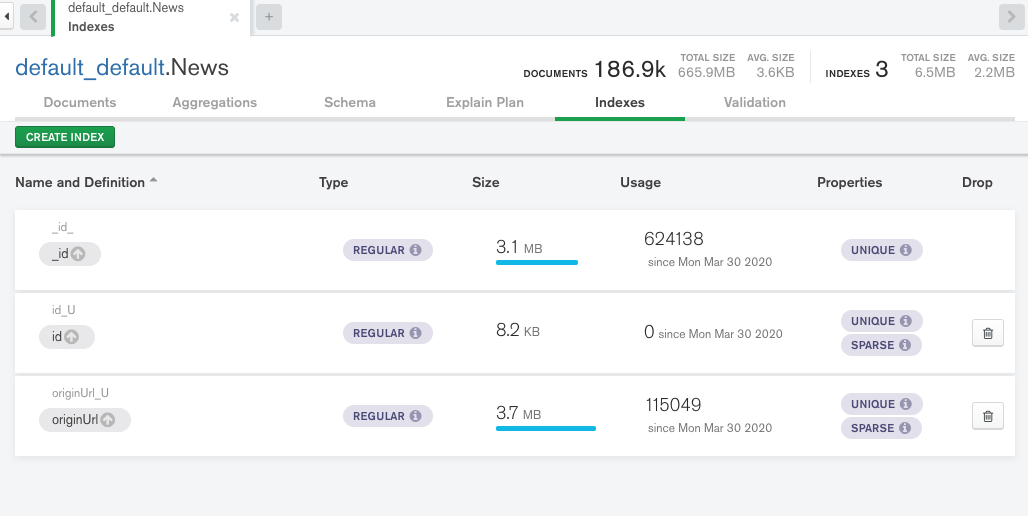
\includegraphics[width=1\linewidth]{pics/mongodb-search-indizes.png}
    \caption{MongoDB Search Index}
    \label{fig:enter-label}
\end{figure}





https://www.atlassearchindexes.com/
https://www.mongodb.com/basics/database-index